\clearpage
\pdfpagewidth=35cm
\pdfpageheight=25cm
\setlength{\textwidth}{34cm}
\setlength{\hsize}{34cm}
\setlength{\oddsidemargin}{\dimexpr(\pdfpagewidth-\textwidth)/2 - 1in\relax}
\setlength{\evensidemargin}{\oddsidemargin}
\setlength{\textheight}{24cm}
\setlength{\vsize}{24cm}
\setlength{\headheight}{0pt}
\setlength{\headsep}{0pt}
\setlength{\topmargin}{\dimexpr(\pdfpageheight-\textheight)/2 - 1in\relax}
\thispagestyle{empty}
\vspace*{0.2cm}
\item Borrar todas las órdenes de la ciudad \textbf{Utah} que tengan artículos de la subcategoría \textbf{Tables}.

\begin{lstlisting}
utah_tables = π orderid (σ state = 'Utah' (customer)
                         ⨝ orders
                         ⨝ σ subcategory = 'Tables' (products))

orders = orders − (orders ⨝ utah_tables)
\end{lstlisting}

La única orden que cumple es \texttt{CA-2015-106320}, que tiene un solo renglón, por lo
que \texttt{orders\_sin\_utah} termina con 5998 renglones.

\vspace{0.35cm}
\centering
\begin{tabular}{@{}c@{\hspace{0.6cm}}c@{}}
	\begin{minipage}[t]{0.38\textwidth}
		\centering
		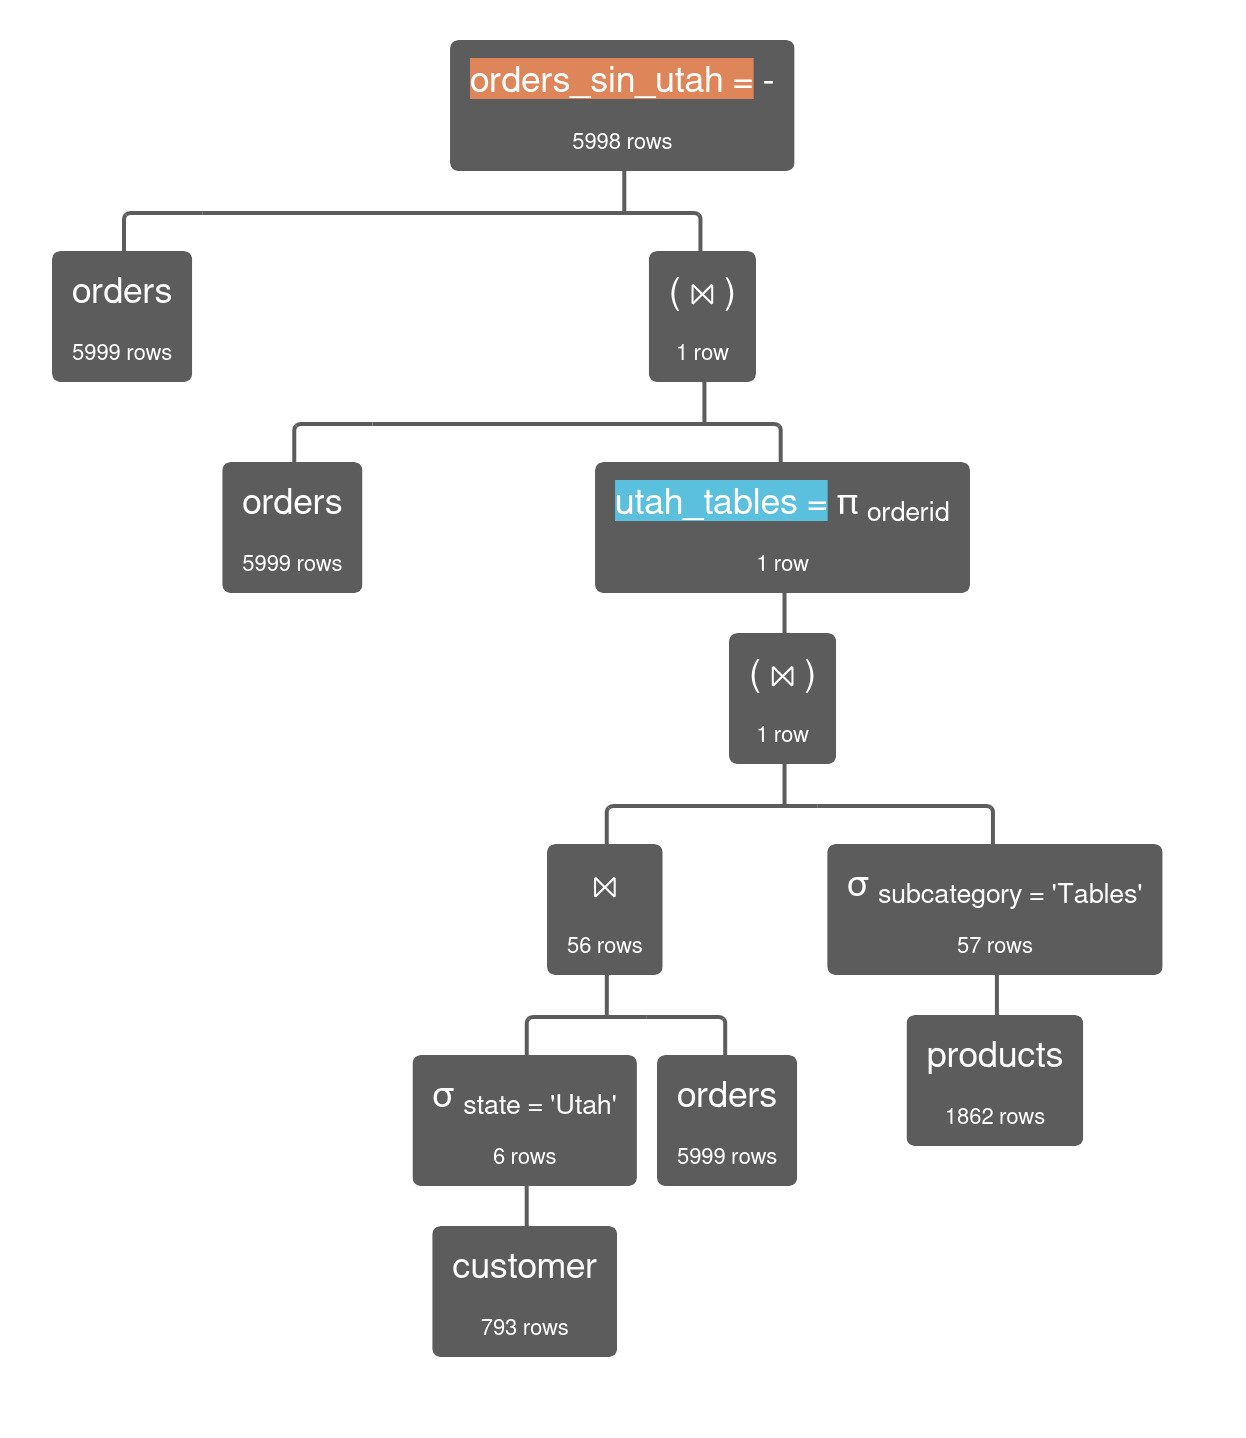
\includegraphics[width=\linewidth]{figuras/3b_arbol.jpg}\\[0.1cm]
		{\small Árbol de \texttt{orders\_sin\_utah}}
	\end{minipage} &
	\begin{minipage}[t]{0.38\textwidth}
		\centering
		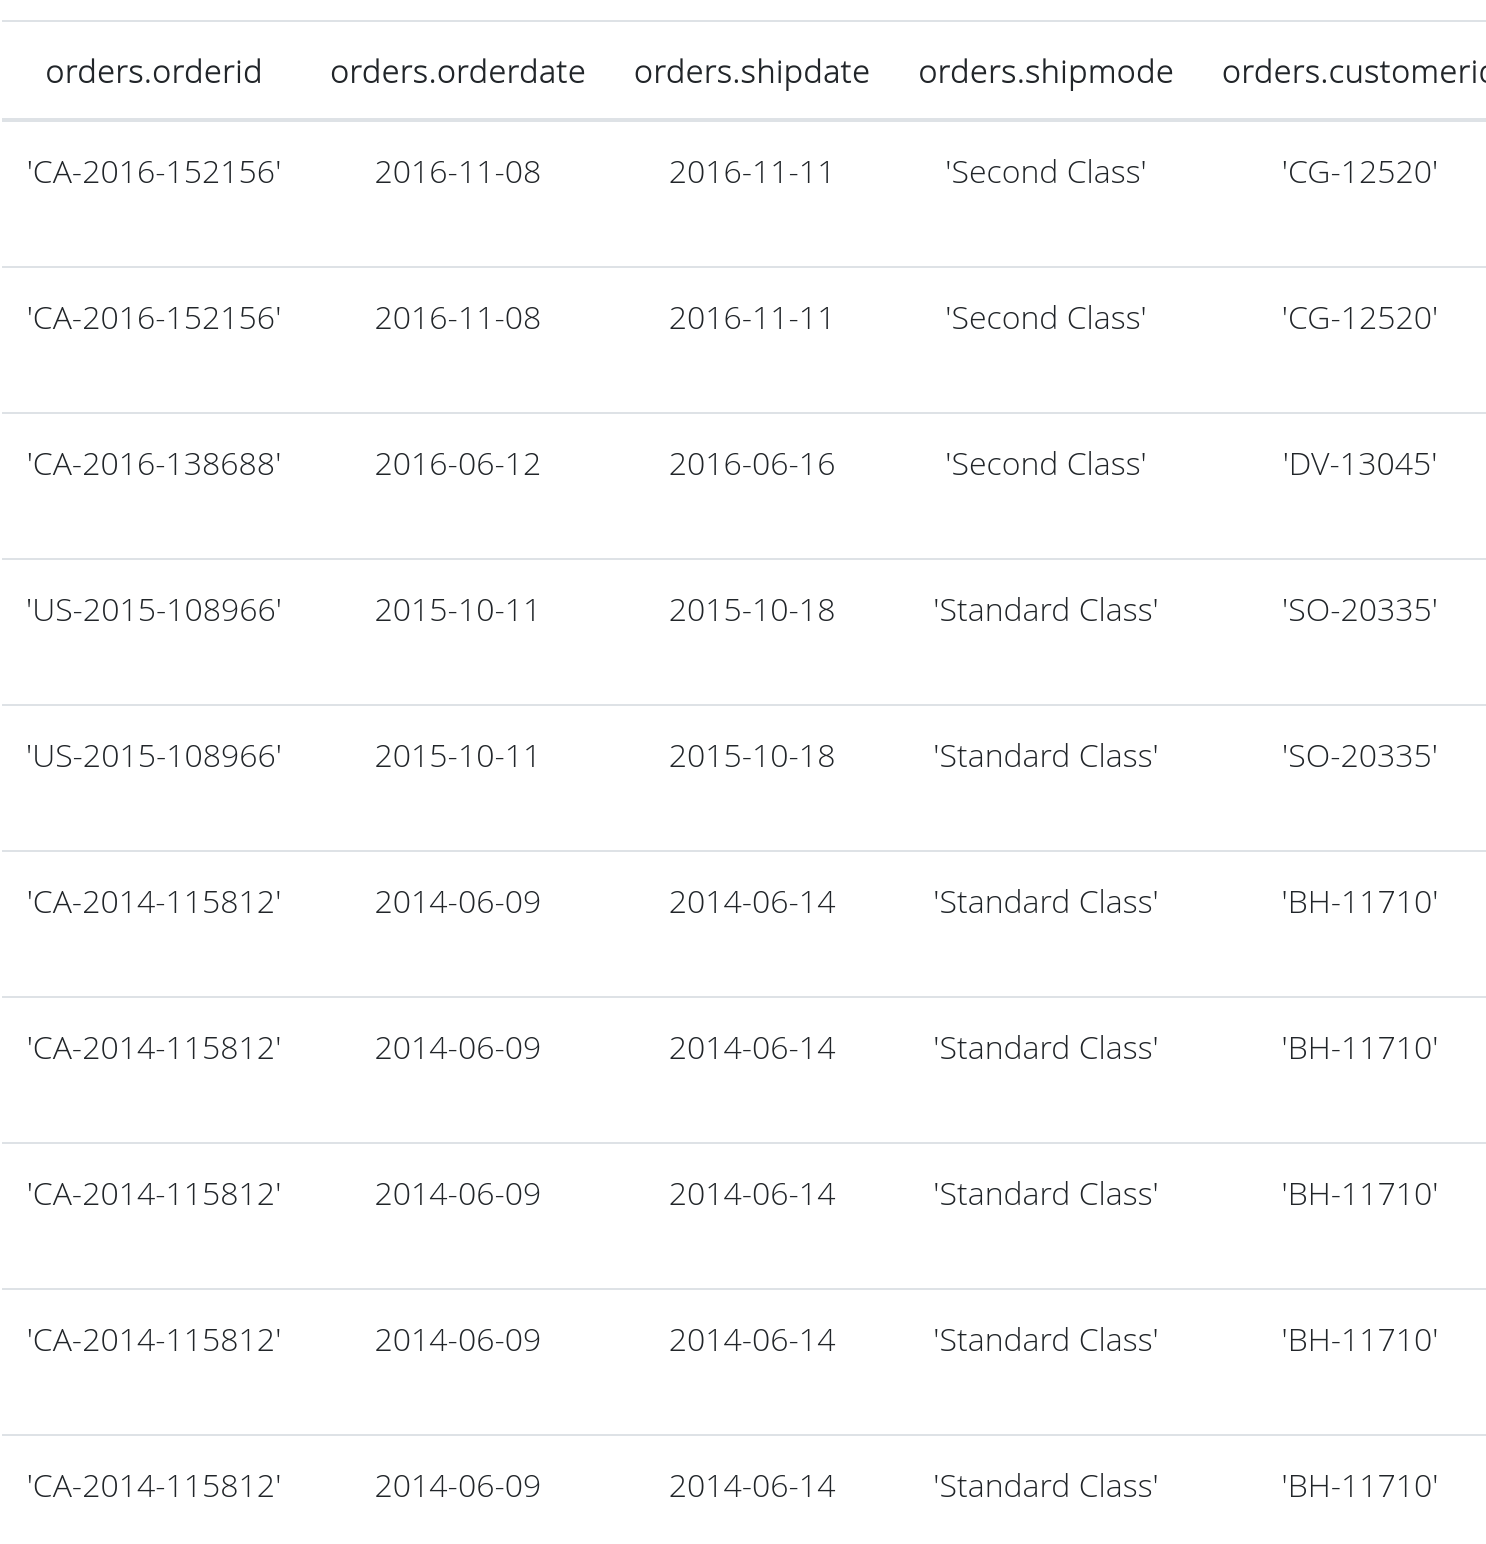
\includegraphics[width=\linewidth]{figuras/3b_tuplas.png}\\[0.1cm]
		{\small Primeros renglones de \texttt{orders\_sin\_utah}}
	\end{minipage}
\end{tabular}

\vspace{0.3cm}
{\small Las tuplas mostradas son los primeros renglones de la relación
	resultante; la orden \texttt{CA-2015-106320} ya no aparece.}
\clearpage
\restoregeometry
\pdfpagewidth=\paperwidth
\pdfpageheight=\paperheight
